
\graphicspath{{Chapter4/Figs/}}

\setcounter{chapter}{7}
\chapter*{Capítulo 4} 
\addcontentsline{toc}{chapter}{Capítulo 4}
\setcounter{figure}{0}
\setcounter{section}{0}

{\LARGE Estudio bioinformático sobre ARN pequeños y su actividad en \textit{A. thaliana}.}

\section{Introducción}

En plantas existen distintos tipos de ARNs pequeños con distintos tamaño que varían de 20 a 25 nucleótidos, origen y mecanismo de acción.
Basado en las diferencias en su biogénesis y su modo de acción, los ARN pequeños de plantas con funciones regulatorias en la expresión génica han sido agrupados en cuatro clases diferentes
\begin{itemize}
	\item siARNs 	(small interfering RNAs) que es la clase más abundante. 
	\item miARNs (microRNAs). De 20 a 22 nt de longitud.
	\item ta-siARN (trans-acting siARNs)
	\item nat-siARNs y nat-miARNs (natural antisense siRNAs y miRNAs)
\end{itemize}

El cambio climático es uno de los temas más importantes para la ciencia en este momento. 
Debido a que las plantas no regulan la temperatura, es posible que una modificación en la temperatura del ambiente pueda cambiar el procesamiento de los miARNs.
Para analizar esto, se realizaron secuenciaciones de alto rendimiento de ARN pequeños de plantas crecidas a diferentes temperaturas.
En estas mismas plantas se secuenciaron bibliotecas de PARE \citep{pmid19247285} para la identificación de genes blanco de miARNs que permite realizar estudios del degradoma de ARN, mediante técnicas de alto rendimiento.
Esto lo hicimos para estudiar como afecta la temperatura a los genes blanco predichos anteriormente y si existen nuevos genes blanco regulados por miARNs a bajas y altas temperaturas.

\section{Resultados y Discusión}

\subsection{Biogénesis y actividad de ARN pequeños de plantas en distintas temperaturas}

\subsubsection{Mapeo y ARN pequeños en condiciones de estrés dependientes de la temperatura}

Primero queríamos estudiar si se modifica la biogénesis y actividad de los ARN pequeños en distintas temperaturas.
Para esto realizamos secuenciación masiva para bibliotecas de plantas de ARNm de \textit{A. thaliana} a baja temperatura (8\degree C), a temperatura normal (22\degree C) y a alta temperatura (37\degree C).

Brevemente, un total de $\sim$ 26 millones, $\sim$ 18 millones y $\sim$ 23 millones de lecturas en promedio fueron secuenciadas para baja temperatura, normal y alta.
Las lecturas fueron filtradas para remover los adaptadores y antes de mapearlas contra el genoma de \textit{A. thaliana}, observamos la distribución del tamaño de las secuencias totales (Figura \label{fig:distribucion_lecturas_totales}.
Las lecturas están normalizadas para poder hacer una comparación cuantitativa de las lecturas.

Observamos una distribución consistente del largo de las secuencias únicas a lo largo de las bibliotecas.
La distribución varía entre 18nt y 30 nt.
También observamos que la mayoría de las lecturas muestran un pico en largos entre 20 y 24 nt, consistente con reportes previos.
El enriquecimiento para las todas las bibliotecas, sin importar la temperatura, está en los de 21 nt y 24 nt (Figura \ref{fig:distribucion_lecturas_totales}).

\begin{figure}[htbp!] 
    \centering    
    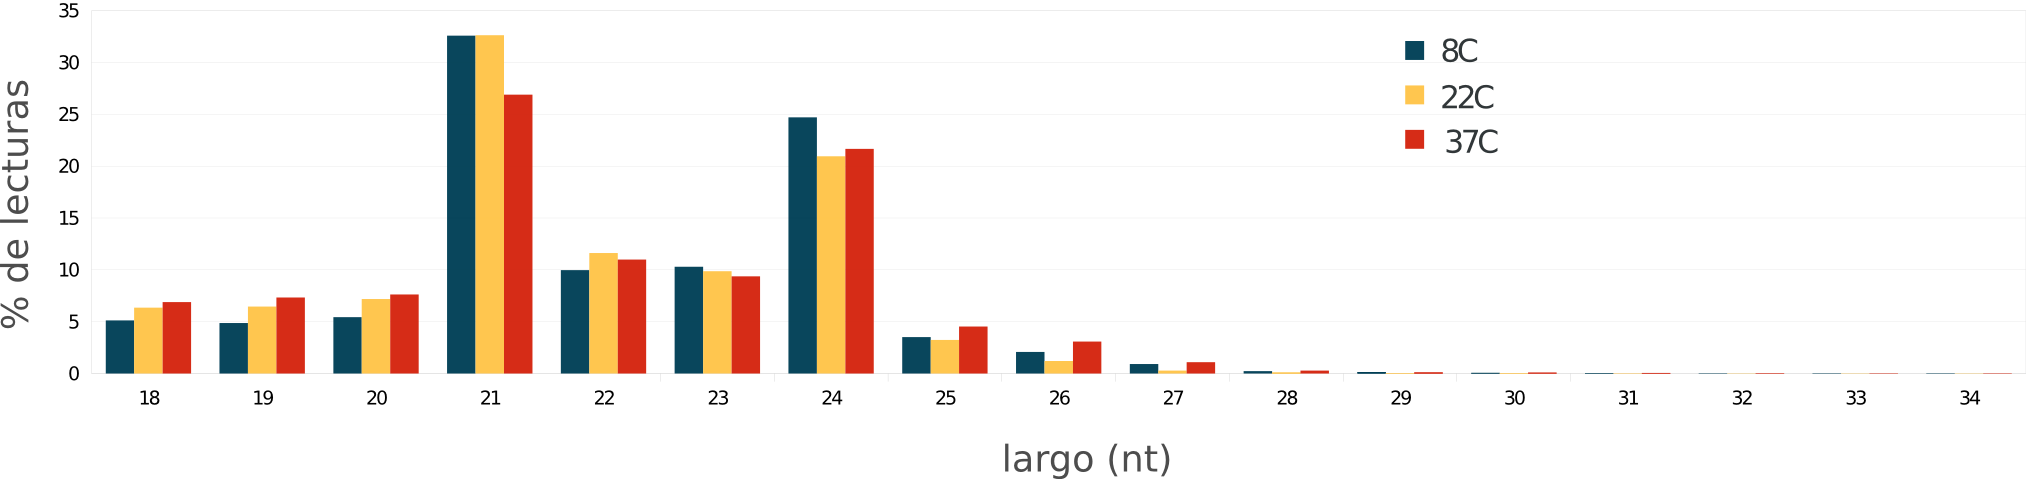
\includegraphics[width=1\textwidth]{distribucion_lecturas_totales.png}
    \caption[Distribución del tamaño de las lecturas totales de ARN pequeños]{
    \textbf{Distribución del tamaño de las lecturas de ARN pequeños}
    Distribución del tamaño de las lecturas totales de ARN pequeños de las 3 bibliotecas secuenciadas (8\degree C, 22\degree C y 37\degree C).
   }
     \label{fig:distribucion_lecturas_totales}
\end{figure}

Luego estás secuencias fueron mapeadas contra los elementos del genoma de \textit{A. thaliana}.
Y por último las lecturas redundantes fueron agrupadas en un dataset y el número de copias de cada lectura fue asignado a una lectura única (etiqueta).
Esto dio como resultado a un conjunto de lecturas no redundantes de $\sim$ 2 millones para 8\degree C, $\sim$ 1,3 millones para 22\degree C y $\sim$ 1,6 millones para 37\degree C, de etiquetas únicas (Tabla \ref{table:sRNA_libraries}).

\begin{table}[!htbp]
\centering
\small
\caption{Bibliotecas de ARN pequeños}
\label{table:sRNA_libraries}
\begin{tabular}{clcccc}
\rowcolor[HTML]{ECF4FF} 
\hline
Código       & Muestras de plantas    & Secuencias totales & \begin{tabular}[c]{@{}c@{}}Lecturas que\\ mapean contra\\ el genoma\end{tabular} & \begin{tabular}[c]{@{}c@{}}Lecturas únicas\\ que mapean\\ contra el genoma\end{tabular}  \\ \hline
col\_8c\_1s  & Muestra 1 a 8°C   & 26594034           & 15235935                                                                         & 2181244                                                                                    \\ \hline
col\_8c\_2s  & Muestra 2 a 8°C   & 24503495           & 14064726                                                                         & 2073756                                                                                       \\ \hline
col\_22c\_1s & Muestra 1 a 22°C  & 13922338           & 6805121                                                                          & 952466                                                                                        \\ \hline
col\_22c\_2s & Muestra 2 a 22°C  & 23037685           & 12430935                                                                         & 1699845                                                                                        \\ \hline
col\_37c\_1s & Muestra 1 a 37°C  & 22273823           & 9109248                                                                          & 1388169                                                                                       \\ \hline
col\_37c\_2s & Muestra 2 a 37°C  & 24307772           & 12748308                                                                         & 1867528                                                                                       \\ \hline
\end{tabular}
\end{table}

Una vez mapeadas las lecturas únicas contra el genoma, observamos nuevamente la distribución del tamaño de las lecturas en las distintas bibliotecas.
Y observamos que la clase más abundante a distintas temperaturas son las secuencias de 21nt (Figura \ref{fig:distribucion_sRNA}), aunque se ve una diferencia poco significativa a 8\degree C, 22\degree C y 37\degree C.

\begin{figure}[htbp!] 
    \centering    
    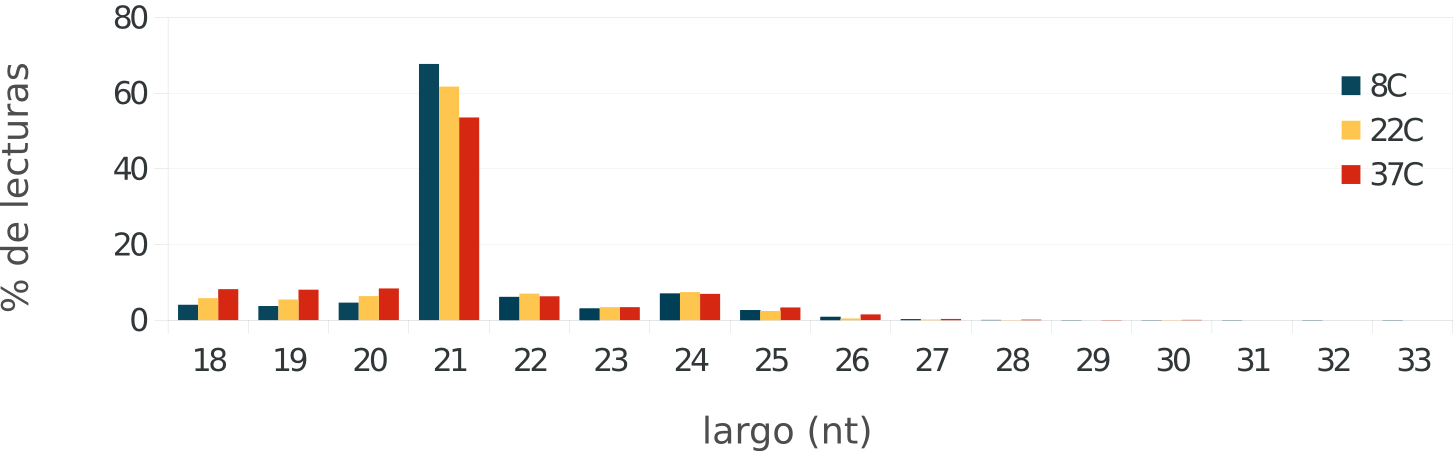
\includegraphics[width=.8\textwidth]{cantidad_lecturas.png}
    \caption[Distribución del tamaño de las lecturas de ARN pequeños que mapean contra el genoma de \textit{A. thaliana}]{
    \textbf{Distribución del tamaño de las lecturas de ARN pequeños que mapean contra el genoma de \textit{A. thaliana}.}
    Distribución del tamaño de las lecturas de ARN pequeños que mapean contra el genoma de \textit{A. thaliana}.
    Se muestra la distribuciín para las 3 bibliotecas secuenciadas (8\degree C, 22\degree C y 37\degree C).
   }
     \label{fig:cantidad_lecturas}
\end{figure}


\subsubsection{Perfil comparativo de ARN pequeños a distintas temperaturas y asignación a través de las características genómicas de \textit{A. thaliana}}

Para las lecturas únicas que mapean contra el genoma de \textit{A. thaliana}, observamos la distribución de estos ARN pequeños a lo largo del mismo (Figura \ref{fig:distribucion_sRNA}).
Observamos que la clase más abundante para las 3 temperaturas era la de ARN ribosomal, donde es mayoritaria en casi el 50\% de las lecturas mapeadas.
Luego aparecen los miARNs y ARN pequeños que pegan contra genes que codifican para proteínas.
Otra de las clases más abundantes fueron los transposones y en menor porcentaje otros ARNs entre ellos ARN pequeños nucleares (Figura \ref{fig:distribucion_sRNA}).

No se observan grandes diferencias en la clasificación de los ARN pequeños más abundantes, aunque cuanto más baja es la temperatura parecería que la clase de elementos transponibles aumentan.
Lo opuesto pasa con los ARNs ribosomales (Figura \ref{fig:distribucion_sRNA}).

\begin{figure}[htbp!] 
    \centering    
    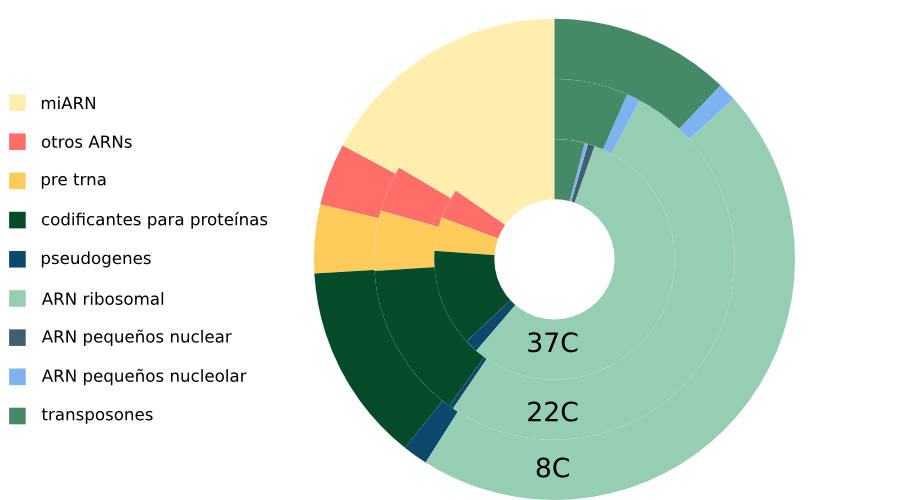
\includegraphics[width=.8\textwidth]{distribucion_sRNA.png}
    \caption[Distribución de ARN pequeños en el genoma de \textit{A. thaliana}]{
    \textbf{Distribución de ARN pequeños en el genoma de \textit{A. thaliana}}
        }
     \label{fig:distribucion_sRNA}
\end{figure}

Entre ellos los más abundantes son miembros de la familia del miR165/166, el miR396 (siendo el miR396b más abundante que el miR396a), el miR398b/c, el miR158, el miR159, el miR156/157, el miR403 y el miR408.
En cuanto a los ARN pequeños identficados como miARNs, se detectaron una gran cantidad de miARNs conocidos.
La tabla completa para miARNs que tienen más de 100 lecturas, sumando todas las bibliotecas juntas, se muestra en la tabla del anexo \ref{table:abundancia_miARN}.

En total nos quedamos con 1271 ARN pequeños de plantas crecidas a 8\degree C, con 1305 ARN pequeños de plantas crecidas a 22\degree C y con 1129 ARN pequeños de plantas crecidas 37\degree C.
Si bien la mayoría de los ARN pequeños encontrados son los mismos en las 3 bibliotecas, existen algunos que sólo se detectaron en dos bibliotecas o en una sola.
Estas diferencias se debe en gran parte al corte arbitrario del número de lecturas que utilizamos para el conjunto de ARN pequeños final.
 
\begin{figure}[htbp!] 
    \centering    
    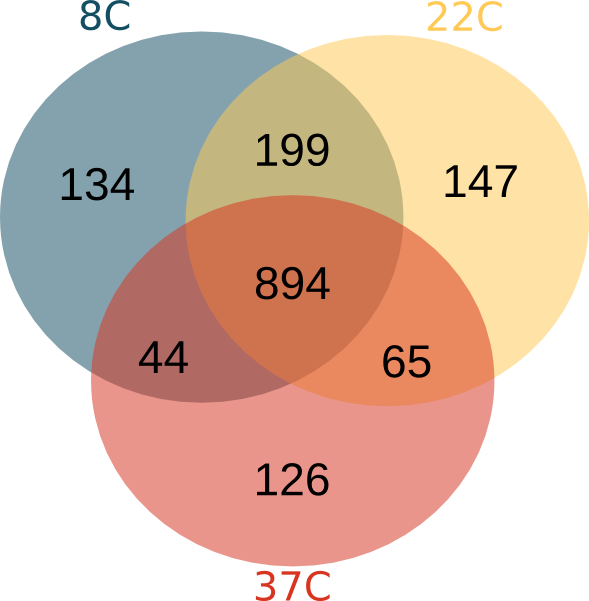
\includegraphics[width=.4\textwidth]{venn_sRNA_abundantes.png}
    \caption[Diagrama de Venn de ARN pequeños más abundantes a diferente temperaturas]{
    \textbf{Diagrama de Venn de ARN pequeños más abundantes a diferente temperaturas}
    }
        
     \label{fig:venn_sRNA_abundantes}
\end{figure}

\subsection{Pipeline automatizado para el análisis genómico de ARN pequeños y su actividad in vivo en plantas}

Además de las bibliotecas de ARN pequeños, utilizamos estás mismas plantas sometidas a estrés en distintas temperaturas para realizar bibliotecas de PARE\citep{pmid19247285}.
La misma permite realizar estudios del degradoma de ARN e identificar fragmentos cortados por miARNs u otros ARN pequeños que causen cortes endonucleolíticos de los ARNm blanco.
Para esto utilizamos una estrategia y desarrollamos un pipeline automatizado para la predicción de genes blanco de ARN pequeños de \textit{A. thaliana} (Figura \ref{fig:sRNA_strategy}).

Utilizamos CleaveLand \citep{pmid19017659}, que es una herramienta computacional para la detección de cortes de miARNs en datos de degradoma.
Cleaveland toma como entrada datos de degradomas, ARN pequeños y una base de datos de ARNm y devuelve genes blanco de ARN pequeños.
En nuestro caso utilizamos todos los ARN pequeños más abundantes mapeados de las bibliotecas a distintas temperaturas que mostramos anteriormente (Figura \ref{fig:sRNA_strategy}).

\begin{figure}[htbp!] 
    \centering    
    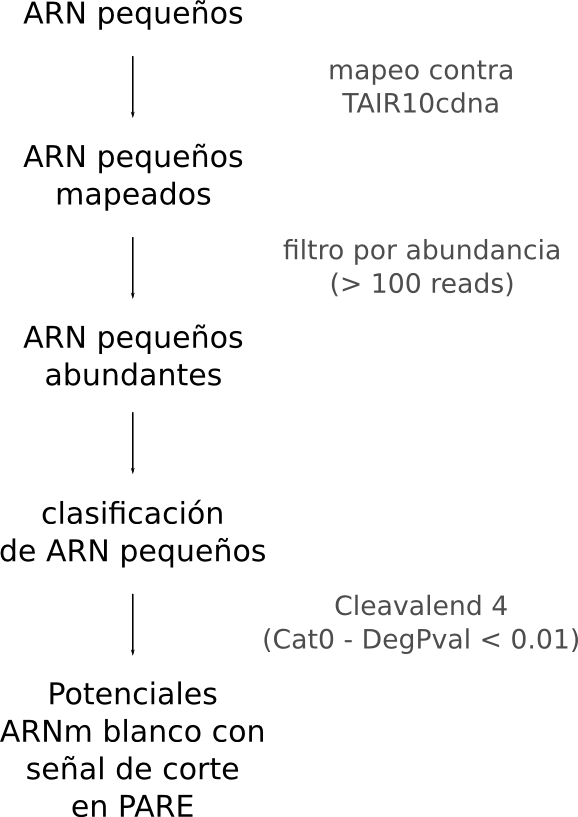
\includegraphics[width=.3\textwidth]{sRNA_strategy.png}
    \caption[Estrategia para el análisis de bibliotecas de ARN pequeños de \textit{A. thaliana}]
    {
    \textbf{Estrategia para el análisis de bibliotecas de ARN pequeños de \textit{A. thaliana}}.
    Las bibliotecas de ARN pequeños fueron filtradas para remover los adaptadores y luego fueron mapeadas contra el genoma de \textit{A. thaliana}.
    Nos quedamos con los ARN pequeños más abundantes (>100 reads en ambas muestras) que luego fueron clasificados.
    Con estos ARN pequeños hicimos una búsqueda sistematizada de potenciales ARNm blanco que tienen señal de corte por PARE.
    }
     \label{fig:sRNA_strategy}
\end{figure}

Los resultados de este pipeline automatizado se muestran en la Figura \ref{fig:sRNA_results}.
De los 1271 ARN pequeños a  8\degree C, se encontraron 78 ARNm con señal por PARE de los cuales son cortados por ARN pequeños que provenien de distintos ARNs: 10 de ARN ribosomal, 1 de genes que codifican para proteínas, 65 por pre-miARNs y 2 por otros ARN pequeños.
A 22 \degree C, se encontraron 67 ARNm con señal por PARE de los cuales son cortados por ARN pequeños que provienen de distintos ARNs: 16 de ARN ribosomal, 1 de genes que codifican para proteínas, 49 por pre-miARNs y 1 por otros ARN pequeños. 
Y a 37 \degree C, se encontraron 65 ARNm con señal por PARE de los cuales son cortados por ARN pequeños que provienen de distintos ARNs: 11 de ARN ribosomal, 1 de genes que codifican para proteínas, 51 por pre-miARNs y 2 por otros ARN pequeños (Figura \ref{fig:sRNA_results}).

Estos resultados son utilizando parámetros de CleaveLand bien estrictos por simplicidad.
Donde por ejemplo solo se consideran los genes blanco con señal en el degradoma que están en la categoria 0 de CleaveLand que significa que tiene más de una lectura y además es la más abundante del transcripto y además es la única mayoritaria.
Esto se hizo para eliminar falsos positivos, pero se podrían relajar los parámetros para obtener mayor cantidad de candidatos y luego estudiarlos en mayor detalle.

\begin{figure}[htbp!] 
    \centering    
    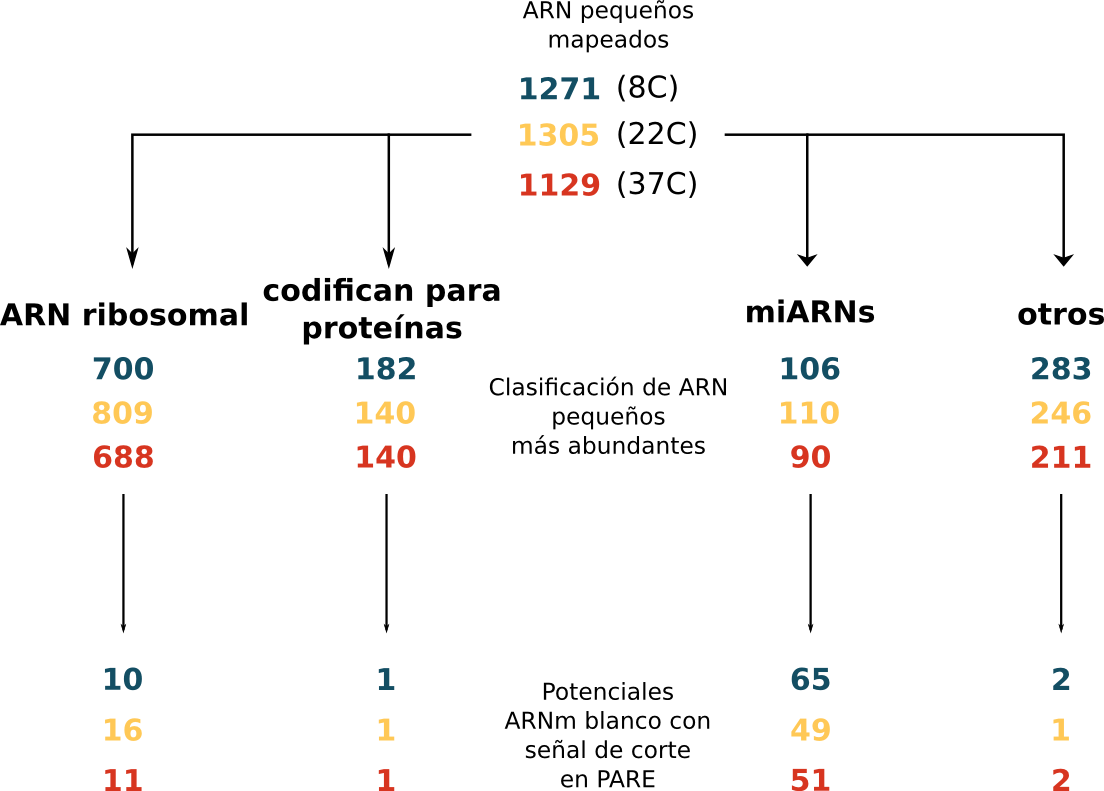
\includegraphics[width=.7\textwidth]{sRNA_results.png}
    \caption[ARNm blanco con señal de corte en PARE a distintas temperaturas]{
    \textbf{ARNm blanco con señal de corte en PARE a distintas temperaturas}
    En color azul se muestran los resultados para los ARN pequeños y potenciales genes blanco en plantas crecidas a 8\degree C.
    En amarillo para plantas crecidas a  22\degree C.
    En rojo para plantas crecidas a  37\degree C.
   }
     \label{fig:sRNA_results}
\end{figure}

Esta misma estrategia puede ser utilizada para encontrar potenciales genes blanco de ARN pequeños en regiones intergénicas o en intrones.
